% !TeX program = xelatex
\documentclass[UTF8,a4paper,11pt,fontset=windows]{ctexart}
\usepackage[left=18mm,right=18mm,top=16mm,bottom=17mm,headheight=14pt]{geometry}
\usepackage{amsmath,amssymb,array,booktabs,longtable,needspace,fancyhdr,xcolor,tikz}
\usepackage[hidelinks]{hyperref}
\setlength{\parindent}{0pt}\setlength{\parskip}{3pt}\linespread{1.1}
\setlength{\emergencystretch}{2em}\raggedbottom
\pagestyle{fancy}\fancyhf{}\renewcommand{\headrulewidth}{0pt}
\fancyfoot[C]{\small\PaperName\quad 第\thepage 页}
\newcommand{\R}{\mathbb R}
\newcommand{\blank}{\underline{\hspace{2.9cm}}}
\newcommand{\src}[1]{\par{\scriptsize\color{black!65}教材改编出处：#1。}\par}
\newcommand{\q}[2]{\par\Needspace{4\baselineskip}\textbf{#1.}\ #2}
\newcommand{\subq}[2]{\par\Needspace{2\baselineskip}（#1）#2}
\newcommand{\opts}[4]{\par\begin{tabular*}{\linewidth}{@{}p{.48\linewidth}@{\extracolsep{\fill}}p{.48\linewidth}@{}}A. #1&B. #2\\C. #3&D. #4\end{tabular*}\par}
\newcommand{\optsfour}[4]{\par\begin{tabular*}{\linewidth}{@{}p{.235\linewidth}@{\extracolsep{\fill}}p{.235\linewidth}p{.235\linewidth}p{.235\linewidth}@{}}A. #1&B. #2&C. #3&D. #4\end{tabular*}\par}
\newcommand{\parttitle}[1]{\par\Needspace{4\baselineskip}{\bfseries #1}\par}
\newcommand{\work}[1]{\par\vspace*{#1}}
\newcommand{\ans}[2]{\par\Needspace{4\baselineskip}\textbf{第#1题}\quad #2\par}
\newcommand{\readinggraph}{\begin{center}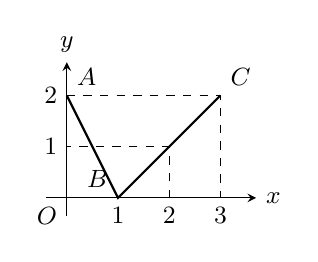
\begin{tikzpicture}[x=.65cm,y=.65cm,>=stealth,font=\small]
\draw[->](-.4,0)--(3.7,0)node[right]{$x$};\draw[->](0,-.35)--(0,2.65)node[above]{$y$};
\draw[thick](0,2)node[above right]{$A$}--(1,0)node[above left]{$B$}--(3,2)node[above right]{$C$};
\draw[dashed](0,2)--(3,2)--(3,0);\draw[dashed](2,0)--(2,1)--(0,1);
\node[below left]at(0,0){$O$};\foreach \x in {1,2,3}\node[below]at(\x,0){$\x$};
\foreach \y in {1,2}\node[left]at(0,\y){$\y$};\end{tikzpicture}\end{center}}
\renewcommand{\arraystretch}{1.2}

\newcommand{\PaperName}{D卷}
\begin{document}
\begin{center}{\Large\bfseries 高一数学期中教材改编练习卷（D）}\\[2mm]湘教版必修第一册\quad 120分钟\quad 满分150分\end{center}
班级\underline{\hspace{2.4cm}}\quad 姓名\underline{\hspace{2.4cm}}\quad 学号\underline{\hspace{2.4cm}}
\parttitle{一、单项选择题（共8小题，每题5分，共40分）}每题只有一个正确选项。
\par\noindent\begin{minipage}{\linewidth}
\q{1}{设全集 $U=\{0,1,2,3,4,5\}$，$A=\{0,2,4\}$，$B=\{1,2,3\}$，则 $A\cap\complement_U B=$（\quad）。}
\optsfour{$\{2\}$}{$\{0,4,5\}$}{$\{0,4\}$}{$\{0,1,2,3,4\}$}
\end{minipage}\par\smallskip
\par\noindent\begin{minipage}{\linewidth}
\q{2}{设 $x\in\R$，则“$x>2$”是“$x>0$”的（\quad）。}
\opts{充分而不必要条件}{必要而不充分条件}{充要条件}{既不充分又不必要条件}
\end{minipage}\par\smallskip
\par\noindent\begin{minipage}{\linewidth}
\q{3}{命题 $p$：$\forall x\in[-1,1]$，$x^2\le1$。则 $p$ 的否定是（\quad）。}
\opts{$\forall x\in[-1,1]$，$x^2>1$}{$\exists x\in\R$，$x^2>1$}{$\exists x\in[-1,1]$，$x^2\ge1$}{$\exists x\in[-1,1]$，$x^2>1$}
\end{minipage}\par\smallskip
\par\noindent\begin{minipage}{\linewidth}
\q{4}{已知 $x>2$，则 $2x+\dfrac8{x-2}$ 的最小值是（\quad）。}
\optsfour{$10$}{$12$}{$8$}{$16$}
\end{minipage}\par\smallskip
\par\noindent\begin{minipage}{\linewidth}
\q{5}{下列各组函数中，表示同一个函数的是（\quad）。}
\opts{$y=x$ 与 $y=\sqrt{x^2}$}{$y=x$ 与 $y=\dfrac{x^2}x$}{$y=x^3$ 与 $y=\sqrt[3]{x^9}$}{$y=\sqrt x$ 与 $y=\sqrt{-x}$}
\end{minipage}\par\smallskip
\par\noindent\begin{minipage}{\linewidth}
\q{6}{函数 $f(x)=\dfrac{\sqrt{2-x}}{x^2-1}$ 的定义域是（\quad）。}
\opts{$(-\infty,-1)\cup(-1,1)\cup(1,2]$}{$(-\infty,2]$}{$(-\infty,-1)\cup(-1,1)\cup(1,2)$}{$(-\infty,-1)\cup(1,2]$}
\end{minipage}\par\smallskip
\par\noindent\begin{minipage}{\linewidth}
\q{7}{已知 $f(x)$ 是定义在 $\R$ 上的偶函数，当 $x\ge0$ 时，$f(x)=x^2+1$，则 $f(-2)-f(1)=$（\quad）。}
\optsfour{$-3$}{$7$}{$5$}{$3$}
\end{minipage}\par\smallskip
\par\noindent\begin{minipage}{\linewidth}
\q{8}{若函数 $f(x)=x^2+2(a+1)x$ 在区间 $[1,+\infty)$ 上单调递增，则 $a$ 的取值范围是（\quad）。}
\optsfour{$(-\infty,-2]$}{$[-2,+\infty)$}{$(-2,+\infty)$}{$(-\infty,-2)$}
\end{minipage}\par\smallskip

\newpage
\parttitle{二、多项选择题（共3小题，每题6分，共18分）}每题有多项正确。全部选对得6分，部分选对且无错项得3分，含错项或未选得0分。
\par\noindent\begin{minipage}{\linewidth}
\q{9}{已知 $a<b$，$c<0$，则下列结论正确的是（\quad）。}
\opts{$ac>bc$}{$a-c>b-c$}{$\dfrac ac>\dfrac bc$}{$a^2>b^2$}
\end{minipage}\par\smallskip
\par\noindent\begin{minipage}{\linewidth}
\q{10}{已知 $f(x)=-(x-1)^2+4$，$x\in[-1,2]$，则下列结论正确的是（\quad）。}
\opts{$f(x)$ 的最大值为4}{$f(x)$ 的最小值为0}{$f(x)$ 在 $[-1,2]$ 上单调递增}{$f(x)$ 的值域为 $[0,4]$}
\end{minipage}\par\smallskip
\par\noindent\begin{minipage}{\linewidth}
\q{11}{已知 $f(x)$ 是定义在 $\R$ 上的偶函数，且在 $[0,+\infty)$ 上单调递减，则下列结论正确的是（\quad）。}
\opts{$f(-3)<f(-1)$}{$f(-2)=f(2)$}{$f(-1)<f(2)$}{$f(0)\le f(1)$}
\end{minipage}\par\smallskip
\parttitle{三、填空题（共3小题，每题5分，共15分）}
\par\noindent\begin{minipage}{\linewidth}
\q{12}{若对任意 $x\in\R$，$x^2-6x+k\ge0$ 恒成立，则 $k$ 的取值范围为\blank。}
\end{minipage}\par\smallskip
\par\noindent\begin{minipage}{\linewidth}
\q{13}{已知函数 $f(x)$ 对任意 $x\in\R$ 都满足 $f(x+2)=2x-1$，则 $f(3)=$\blank。}
\end{minipage}\par\smallskip
\par\noindent\begin{minipage}{\linewidth}
\q{14}{函数 $f(x)=|x-1|-|x-3|$ 的值域为\blank。}
\end{minipage}\par\smallskip
\parttitle{四、解答题（共5小题，共77分）}解答须写出文字说明、证明过程或演算步骤。
\q{15}{（15分）设全集 $U=\R$，集合 $A=\{x\mid-1\le x\le3\}$，$B=\{x\mid t<x\le5\}$，其中 $t<5$。\subq{1}{当 $t=1$ 时，求 $A\cap B$、$A\cup B$ 和 $\complement_U A$；}\subq{2}{若 $A\cup B=[-1,5]$，求 $t$ 的取值范围。}}
\work{4.0cm}

\newpage
\q{16}{（15分）解下列关于 $x$ 的不等式，其中 $m\in\R$。\subq{1}{$2x^2+x-3<0$；}\subq{2}{$x^2-(m-2)x-2m\le0$。}}
\work{6.7cm}
\q{17}{（17分）已知函数 $g(x)$ 的定义域为 $[-3,3]$，设 $f(x)=g(x)+g(-x)$，且当 $x\in[0,3]$ 时，$f(x)=x^2-2x+3$。\subq{1}{判断 $f(x)$ 的奇偶性，并证明；}\subq{2}{求 $f(x)$ 在 $[-3,0)$ 上的解析式；}\subq{3}{用定义证明 $f(x)$ 在 $[1,3]$ 上单调递增，并求 $f(x)$ 在 $[-3,3]$ 上的最大值、最小值及取得相应最值时 $x$ 的所有取值。}}
\work{7.0cm}

\newpage
\q{18}{（17分）完成下列问题。\subq{1}{计算 $64^{\frac23}-16^{-\frac12}$；}\subq{2}{已知幂函数 $f(x)=x^\alpha$ 的图象经过点 $\left(9,\dfrac13\right)$，求其解析式及定义域；}\subq{3}{判断（2）中函数的奇偶性，写出其单调区间，并用定义证明其单调性。}}
\work{6.6cm}
\q{19}{（13分）已知指数函数 $f(x)=a^x$ 的图象经过点 $(2,4)$，其中 $a>0$ 且 $a\ne1$，令 $h(x)=f(x)-2$。\subq{1}{求 $a$ 的值和 $h(x)$ 的解析式；}\subq{2}{判断 $h(x)$ 的单调性，求其值域和零点；}\subq{3}{解不等式 $h(x)\le6$。}}
\work{6.5cm}
\end{document}
